\documentclass[10pt,letterpaper]{article}
\usepackage[margin=0.8in]{geometry}
\usepackage{booktabs}
\usepackage{graphicx}
\usepackage{amsmath}

\graphicspath{{../output/brief/}}
\setlength{\parskip}{2pt plus 1pt minus 1pt}
\setlength{\parindent}{0pt}

\title{\vspace{-1.5cm}\textbf{Do Withdrawal Cascades Exist in U.S.\ Interconnection Queues?}\vspace{-0.3cm}}
\author{}
\date{\small LBNL Queued Up 2025 --- Internal Progress Report, April 2026}

\begin{document}
\maketitle
\thispagestyle{empty}

\section*{Overview}

When a generation project withdraws from the interconnection queue, shared network upgrade costs are reallocated to the remaining projects at that point of interconnection (POI). In principle, this creates a cascade mechanism: one withdrawal raises costs for neighbors, prompting further withdrawals. This report presents an empirical test of whether that mechanism operates in practice, using 36{,}441 queue requests from the LBNL ``Queued Up'' 2025 dataset.

Two findings frame the analysis. First, \textbf{withdrawals cluster at POIs far more than chance can explain}: the observed variance ratio of POI-level withdrawal rates is 1.63, roughly 31 standard deviations above a permutation null distribution. Second, a \textbf{matched difference-in-differences} design---our strongest causal test---finds no immediate cascade but detects a modest delayed effect emerging 1--2 years after a peer withdrawal, consistent with the institutional timelines for formal restudy and cost reallocation. The cross-sectional signals are overwhelming; the causal signal is modest. Our read is that shared POI-level conditions dominate the observed clustering, with a real but small cascade effect layered on top.

\section*{1. POI Clustering Is Not Chance}

\textbf{Overdispersion.} The variance ratio (observed / expected under independence) of POI-level withdrawal rates is 1.633 across 5{,}278 multi-project POIs ($\chi^2 = 9{,}461.66$, df $= 5{,}277$, $p < 10^{-15}$). A permutation test that shuffles POI labels within entity-year bins places the observed statistic 31 SDs above the null mean (Figure~3). Clustering of this magnitude cannot arise by chance.

\textbf{Cross-sectional logistic regression.} Projects co-located with peers that have withdrawn are dramatically more likely to withdraw themselves. Controlling for capacity, entity, technology, state, and year, the odds ratio for peer withdrawal rate is 10.56 (95\% CI [9.28, 12.02], $p < 0.001$; $N = 16{,}096$). The effect is positive in all 19 testable entities, ranging from 2.10 (NYISO) to 39.9 (WAPA-IS)---a strikingly consistent nationwide pattern. A gradient boosting model achieves cross-validated AUC $= 0.856$ with peer withdrawal count as the top feature by SHAP importance.

\textbf{Dose-response.} Within-depth-bin logistic models (Figure~4) show a monotonically increasing effect: OR rises from 8.9 at 2-project POIs to 72 at 10+ project POIs. A calibrated zero-contagion simulation cannot reproduce the observed coefficients at any depth bin in 1{,}000 replications. These results are descriptive---they cannot by themselves separate genuine peer effects from shared POI-level conditions that drive both the trigger and subsequent withdrawals.

\section*{2. Matched Difference-in-Differences: The Causal Workhorse}

To sharpen identification we match each POI experiencing a first withdrawal (after two clean quarters) to a control POI in the same entity, with the same dominant technology, similar depth, and no recent withdrawals. We obtain \textbf{976 matched pairs} (95.6\% match rate) with excellent covariate balance (all standardized differences $\leq 0.10$). The \textbf{parallel-trends test passes} ($F = 0.47$, $p = 0.71$), supporting the DiD assumption.

\textbf{Event study (Figure~1).} The pooled 4-quarter DiD is null ($-0.008$, $p = 0.73$). The event-time coefficients reveal structure:

\begin{itemize}
\setlength\itemsep{1pt}
\item \textbf{$k = 1$:} significantly \emph{negative} ($-0.038$, $p = 0.009$).
\item \textbf{$k = 4$--$8$:} significantly positive at several horizons (peak $+0.029$, $p = 0.004$), averaging 2--3 percentage points on the quarterly withdrawal probability.
\end{itemize}

The \textbf{delayed-positive pattern is the central causal finding}. It survives restriction to different-developer events (peak $+0.026$, $p = 0.009$) and no-batch events (peak $+0.031$, $p = 0.004$), and it is consistent with formal cost reallocation: interconnection restudies on the relevant entities typically complete 6--18 months after a trigger withdrawal, so we should not expect an instantaneous response.

The $k = 1$ \emph{negative} is new and worth flagging. One potential reading is a short wait-and-see period before developers react to the new cost picture, but we hold this interpretation loosely---alternatives include a conditional-survivor effect in the treated pool or a matching artifact. The pattern is small and is followed by the delayed-positive coefficients a year out, so we do not view it as a threat to the main finding, but we make no strong claim about its mechanism.

\section*{3. The Cox Signal Is Depth-Dependent}

Our time-varying Cox model (counting-process format, 7{,}926 subjects, 3{,}930 events) returns a \emph{null} hazard ratio at depth $\geq 2$ (HR $= 1.011$, [0.995, 1.028], $p = 0.18$)---a downgrade from an earlier version reporting HR $\approx 1.032$, after fixing a counting-process bug that mechanically admitted $\sim$1{,}350 same-day peer exposures and merging 1{,}463 duplicate POIs via improved name normalization.

The pooled null is \textbf{also partly mechanical}: the depth-$\geq 2$ sample is dominated by 2-project POIs where \texttt{cumulative\_peer\_wd} has no within-subject variation---it is 0 then 1 and never changes again. Restricting to deeper POIs recovers a significant effect:

\begin{center}
\small
\begin{tabular}{lccc}
\toprule
Sample & HR (cum.\ peer\_wd) & 95\% CI & $p$ \\
\midrule
Depth $\geq 2$ & 1.011 & [0.995, 1.028] & 0.18 \\
Depth $\geq 3$ & \textbf{1.023} & [1.005, 1.041] & 0.011 \\
Depth $\geq 5$ & \textbf{1.029} & [1.008, 1.050] & 0.007 \\
\bottomrule
\end{tabular}
\end{center}

We read this as: \emph{the temporal contagion is identifiable wherever POIs are deep enough to generate repeated peer exposure}, mirroring the dose-response pattern in the cross-section.

\textbf{Proportional hazards fails.} A time-interaction test rejects PH for \texttt{cumulative\_peer\_wd} ($p = 0.0001$), and a calendar split confirms it: early-period HR $= 0.954$ ($p < 0.001$), late-period HR $= 1.005$ ($p = 0.69$). The effect is not constant over time. We do not have a clean story for the early-period sub-unity coefficient---it may reflect baseline-hazard secular trends---but the point is that \textbf{any single pooled hazard ratio is misleading}, and we report depth-stratified estimates.

\section*{4. Upper Bound, Caveats, and Synthesis}

\textbf{Strict-control upper bound.} Restricting controls to POIs that \emph{never} experienced a withdrawal (873 pairs) yields much larger coefficients: $+0.068$ at $k = 1$ ($p \approx 6\times 10^{-13}$), $+0.057$ at $k = 4$, $+0.049$ at $k = 7$. We treat this as an \textbf{upper bound}, not the main result: requiring controls to have zero withdrawals across the entire window conditions on a post-treatment outcome and enforces hard selection---``ever-withdrew vs.\ never-withdrew'' rather than ``exposed now vs.\ not-yet-exposed.'' The 976-pair match is the correct causal contrast; the strict-control number bounds how much of the total clustering is between ``bad-site'' and ``good-site'' POIs. Measurement error in POI names likely attenuates all estimates despite aggressive normalization.

\textbf{Synthesis.} POI-level clustering is the dominant feature of the data. The cross-sectional OR of ${\sim}$10.6 combines shared site conditions and peer effects and cannot by itself apportion the two. The cleanest causal evidence for a cascade channel is the matched DiD's delayed-positive pattern at 4--8 quarters ($+2$--$3$ pp), surviving multiple sensitivity checks and parallel pre-trends. The Cox model supports this picture at deeper POIs but not in pooled form, and the PH violation warns that the effect is not constant. The data support a real cascade mechanism, but its average magnitude is \textbf{modest relative to the cross-sectional clustering}.

For the planned agent-based model: a two-channel specification. \textbf{(i)} Heterogeneous POI-level cost/quality shocks as the dominant source of withdrawal correlation; \textbf{(ii)} a modest cascade multiplier activating with a 12--18 month delay, plausibly period-varying to accommodate the PH violation.\footnote{A Granger-style temporal asymmetry test is not reported. Regressing within-POI late-period withdrawal intensity on early-period intensity (and vice versa) in the new results yields backward $>$ forward, but the OLS asymmetry is driven by the variance of the regressor on each side ($\hat\beta_{fwd} = \mathrm{cov}/\mathrm{var}(\text{early})$ vs.\ $\hat\beta_{bwd} = \mathrm{cov}/\mathrm{var}(\text{late})$); saturated late periods mechanically produce backward-heavy coefficients regardless of causal direction. We consider the test uninformative.}

\clearpage

\begin{figure}[t]
\centering
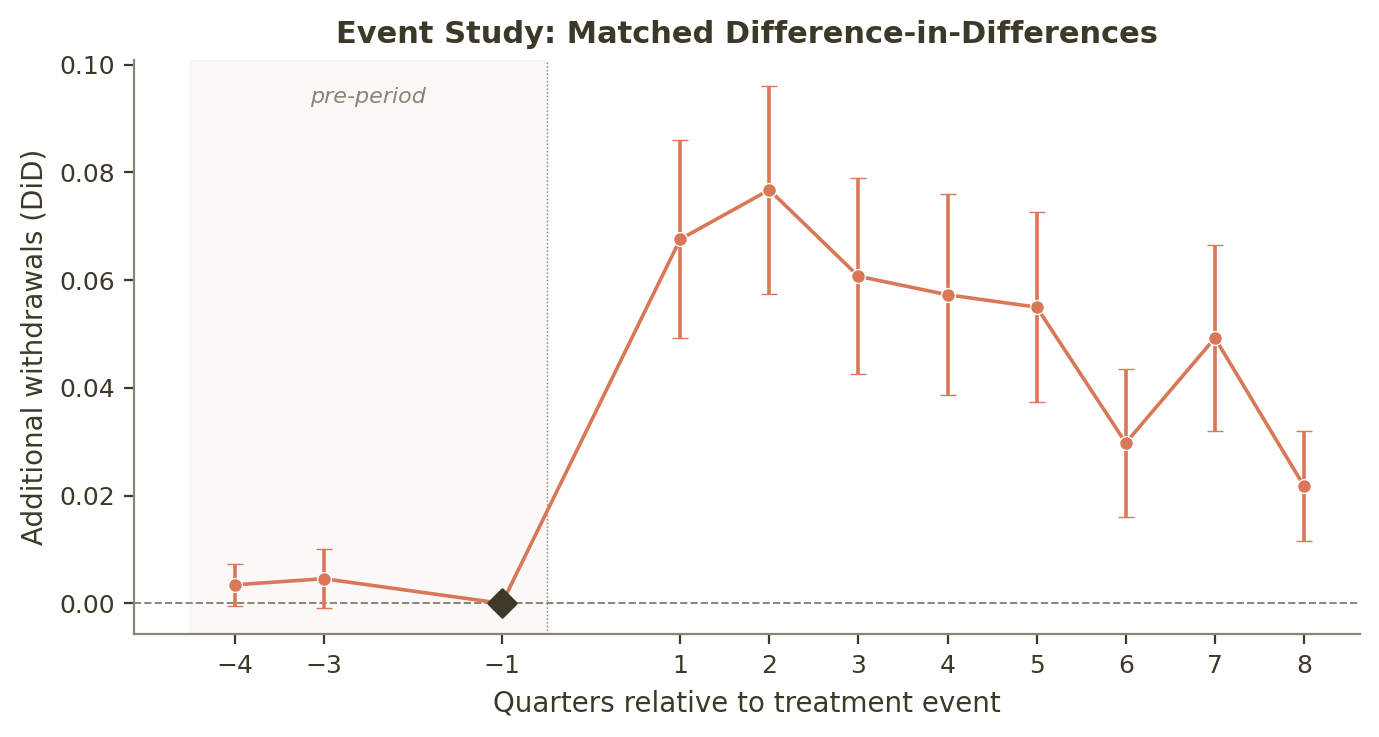
\includegraphics[width=0.72\textwidth]{event_study.png}
\par\smallskip
\small\textbf{Figure 1.} Event-study estimates from matched DiD (976 pairs). Parallel pre-trends ($F = 0.47$, $p = 0.71$). A negative $k{=}1$ dip is followed by significant positive effects at $k = 4$--$8$ quarters (1--2 years), consistent with formal cost-reallocation timelines.
\end{figure}

\begin{figure}[h]
\centering
\begin{minipage}{0.32\textwidth}
\centering
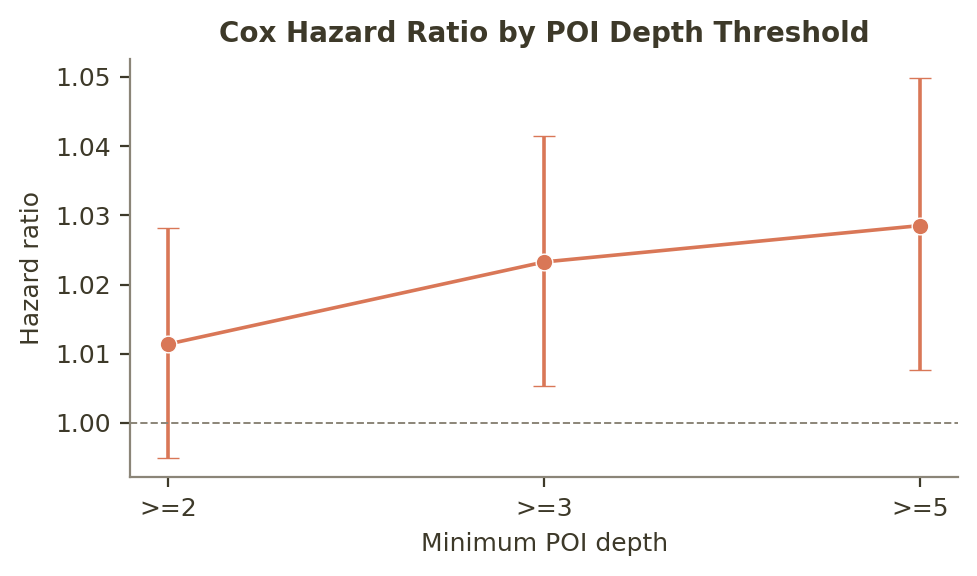
\includegraphics[width=\textwidth]{cox_depth.png}
\par\smallskip
\small\textbf{Figure 2.} Cox HR by minimum POI depth. Null at $\geq 2$; significant at $\geq 3$ and $\geq 5$.
\end{minipage}\hfill
\begin{minipage}{0.32\textwidth}
\centering
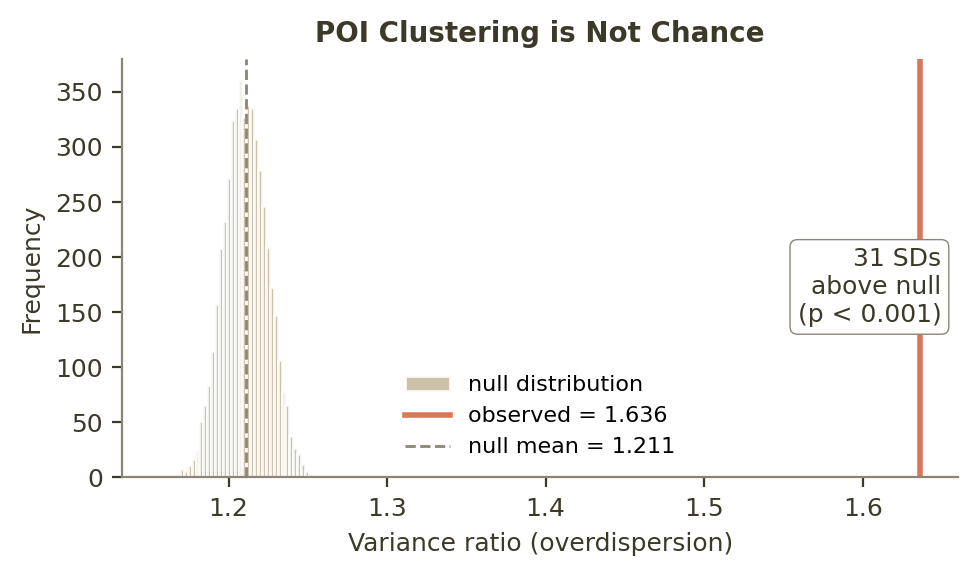
\includegraphics[width=\textwidth]{permutation_null.png}
\par\smallskip
\small\textbf{Figure 3.} Permutation null for POI overdispersion. Observed VR $= 1.63$ sits $\sim$31 SDs above null. 1{,}000 permutations.
\end{minipage}\hfill
\begin{minipage}{0.32\textwidth}
\centering
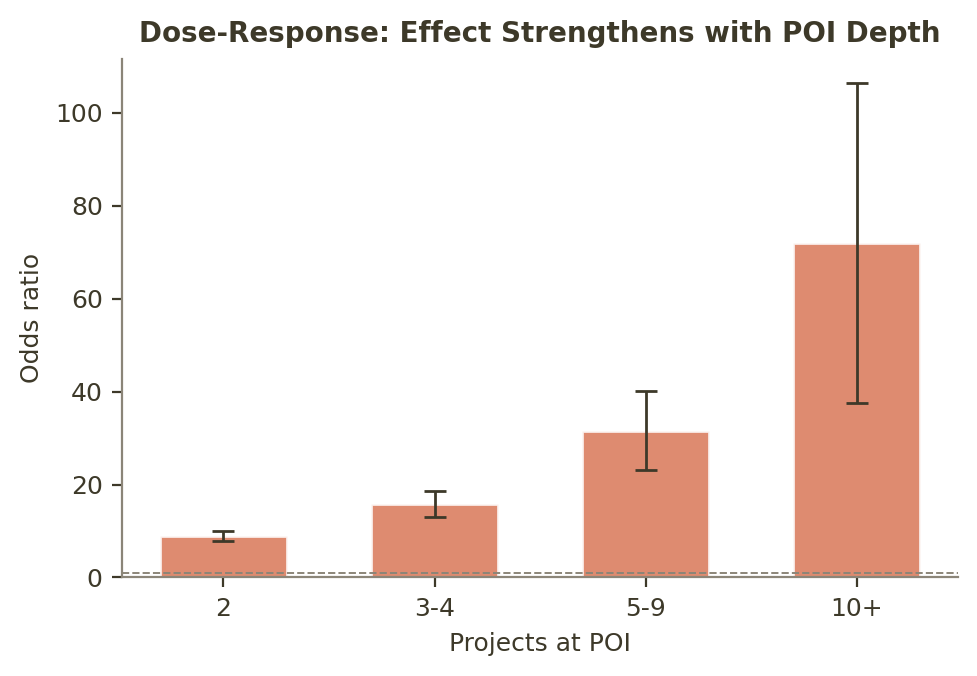
\includegraphics[width=\textwidth]{dose_response.png}
\par\smallskip
\small\textbf{Figure 4.} Dose-response: logistic OR rises from 8.9 at depth 2 to 72 at depth 10+. Zero-contagion simulation cannot reproduce these in 1{,}000 reps.
\end{minipage}
\end{figure}

\end{document}
